\section{Overview}

This tutorial provides an introduction and a very brief overview over how to estimate divergence times and time calibrated phylogeny. 
The key concepts of this tutorial are the global molecular clock and node- and fossil-calibrations.
We have later tutorials that will cover each topic more in detail.
For example, more options on node calibrations are covered in the Node-Calibration tutorial.


In this tutorial you will perform a Bayesian inference to estimate a time-calibrated phylogeny.
In the first part we will demonstrate you how to set up a basic model for time-calibrated phylogeny inference.
There we will use the global molecular clock rate to calibrate the phylogeny.
The first analysis will use a fixed global molecular clock and the second analysis will use an informative prior distribution on the global molecular clock. 
In the second part you will use an informative prior distribution on the root age (crown age) to calibrate the phylogeny.
In the third and final part you will use node- and fossil-calibrations instead of the informative prior on the root age.
All the assumptions will be covered more in detail later in this tutorial.

\subsection*{Requirements}
We assume that you have read and hopefully completed the following tutorials:
\begin{itemize}
\item RB\_Getting\_Started
\item RB\_Basics\_Tutorial
\item RB\_CTMC\_Tutorial
\end{itemize}
Note that the RB\_Basics\_Tutorial introduces the basic syntax of \Rev~but does not cover any phylogenetic models.
You may skip the RB\_Basics\_Tutorial if you have some familiarity with \R.
We tried to keep this tutorial very basic and introduce all the language concepts on the way.
You may only need the RB\_Basics\_Tutorial for a more in-depth discussion of concepts in \Rev.


%%%%%%%%
%%   Data   %%
%%%%%%%%
\section{Data and files}\label{Sec:data}

We provide the data file of DNA sequences required for this tutorial.
You may want to use your own data instead.

\noindent \\ \impmark Create a folder called \cl{data} and download the following files:
\begin{itemize}
\item \href{http://rawgit.com/revbayes/revbayes_tutorial/master/RB_DivergenceTime_Tutorial/data/primates_cytb.nex}{\cl{primates\_cytb.nex}}: Alignment of the \textit{cytochrome b} subunit from 23 primates representing 14 of the 16 families (\textit{Indriidae} and \textit{Callitrichidae} are missing).
\end{itemize}

Below you will also find a table with the calibration dates that we will use later in this tutorial (see Table~\ref{primateFossilTable}).

\begin{table}[tbh!]
\centering
\caption{Node information used for calibrating divergence times in the primate tree.}\label{primateFossilTable}
\begin{tabular}{@{\extracolsep{\fill}}l  c c c r}
\hline
\multicolumn{1}{@{}l}{\textbf{Clade}}  & &\multicolumn{1}{c}{\textbf{Age range (My)}}  & &\multicolumn{1}{c}{\textbf{Citation}} \\ 
\hline
\textit{Simiiformes} & \hspace{2mm} & 43 $\pm$ 4.5 & \hspace{2mm} & \cite{Seiffert2003}\\
\textit{galagids and lorisids} & & 40 $\pm$ 3 &  & \cite{Franzen2009,Poux2004}\\
\hline
\end{tabular}
\end{table}

%
%\subsection*{Analysis Functions}
%
\newpage
\FloatBarrier
\section{Example: Divergence time estimation using a strict, global clock and an informative prior of the clock rate}

\bigskip
\subsection{Getting Started}



The first section of this exercise involves:
(1) setting up a general time reversible (GTR) substitution model \citep{Tavare1986} with gamma distributed rate variation among sites \citep{Yang1994a} for an alignment of the cytochrome b subunit;
(2) use an informative prior on the clock rate to date the phylogeny;
(3) approximating the posterior probability of the tree topology and node ages (and all other parameters) using MCMC, and; 
(4) summarizing the MCMC output by computing the maximum \textit{a posteriori} tree. 
This analysis is mostly equivalent to the analysis performed in the RB\_CTMC\_Tutorial.

\begin{figure}[h!]
\centering
\fbox{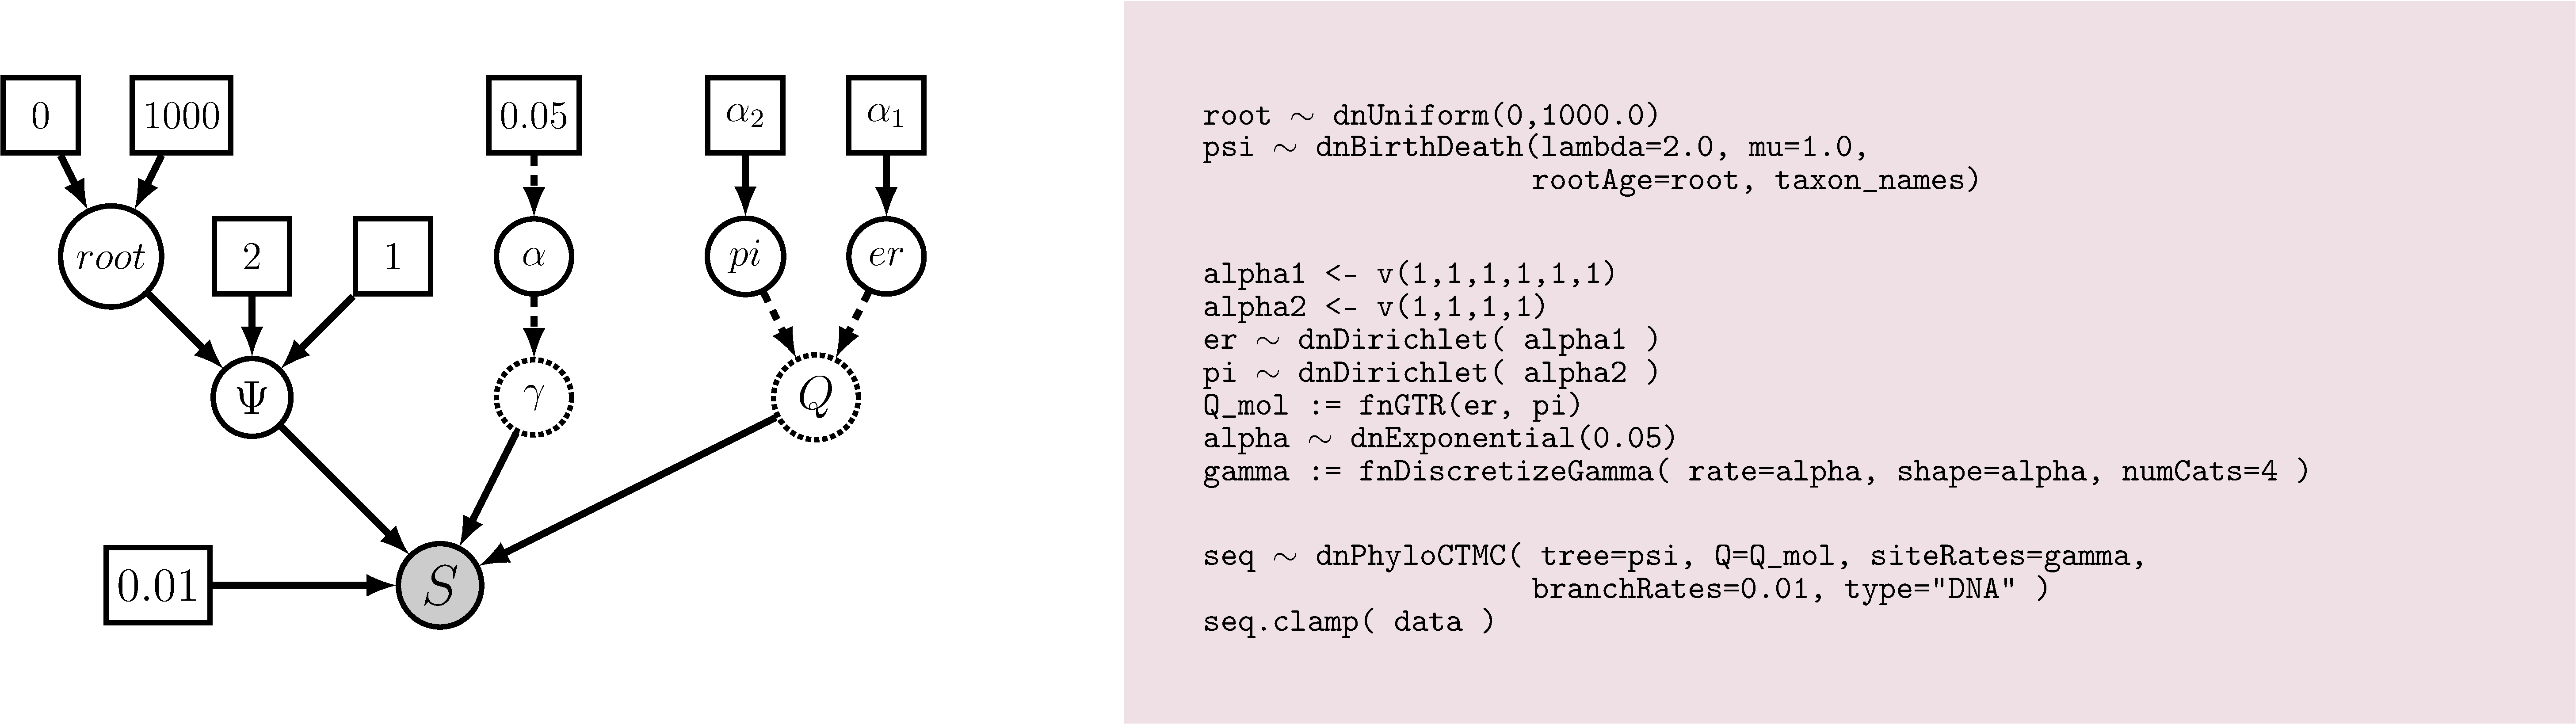
\includegraphics[width=\textwidth,angle=0]{\ResourcePath figures/global_clock_graphical_model.pdf}}
\caption{\small A simple phylogenetic model depicted in graphical-model notation (left) and the corresponding specification in the \Rev~language (right).
In graphical-model notation, constant variables are enclosed in boxes, stochastic variables are enclosed in solid circles, deterministic variables in stippled circles, and observations in shaded circles, with arrows indicating variable dependencies. 
For example, the root age ($root$) is a random variable described by a uniform prior probability distribution with constant upper and lower bounds, the instantaneous-rate matrix, $Q$, is a deterministic function of the base frequencies and exchangeability rates ($pi$ and $er$, respectively), and the observed sequences, $S$, are realizations of the phylogenetic model that are clamped for inference. 
This model is mirrored in \Rev~code, where the first two lines create the birth-death process (with fixed speciation and extinction rates; \emph{lambda}=2.0 and \emph{mu}=1.0), and a uniform prior distribution on the root age. 
The following three lines instantiate the instantaneous-rate matrix for the GTR model, where both the base frequencies and exchangeability rates are drawn from flat Dirichlet distributions.
Finally, we create the stochastic variable representing the character data drawn from the Phylo-CTMC (continuous time Markov chain) process and attach (clamp) observations to the variable \emph{seq}.}
\label{fig:clock_prior}
\end{figure}

The general structure of the model is represented in Figure~\ref{fig:clock_prior}.
This figure shows the full model graph.


\bigskip

\subsection{Loading the Data}

\noindent \\ \impmark You should have already downloaded the data files in Section \ref{Sec:data}. Links to additional files, including the scripts to run these analyses can be found on the \href{http://revbayes.github.io/tutorials.html}{\RevBayes~tutorials website}. Remember that the data file should be in a directory called \cl{data} that is in your current working directory.

First load in the sequences using the \cl{readDiscreteCharacterData()} function. 
%This function returns a \textit{vector} of data matrices and, even though there is only one element in the vector, we must index that element using the \cl{[1]} notation. 
%(You will also note that list indexing in Rev starts with \cl{1} like in the R language.)
{\tt \begin{snugshade*}
\begin{lstlisting}
data <- readDiscreteCharacterData("data/primates_cytb.nex")
\end{lstlisting}
\end{snugshade*}}
Executing these lines initializes the data matrix as the respective \Rev~variable. 

Next we will specify some useful variables based on our dataset. The variable \cl{data} has \textit{member functions} that we can use to retrieve information about the dataset. 
These include the number of species (\cl{n\_species}) and the tip labels (\cl{names}).
Each of these variables will be necessary for setting up different parts of our model (\EG the birth-death process prior).
{\tt \begin{snugshade*}
\begin{lstlisting}
n_species <- data.ntaxa()
names <- data.names()	
\end{lstlisting}
\end{snugshade*}}

Additionally, we set up a counter variable for the number of moves that we already added to our analysis.
[Recall that moves are algorithms used to propose new parameter values during the MCMC simulation.]
This will make it much easier if we extend the model or analysis to include additional moves or to remove some moves.
{\tt \begin{snugshade*}
\begin{lstlisting}
mi = 0 
\end{lstlisting}
\end{snugshade*}}
You may have noticed that we used the \cl{=} operator to create the move index.
This simply means that the variable is not part of the model.
You will later see that we use this operator more often, \EG when we create moves and monitors.

With the data loaded, we can now proceed to specify our substitution model.



\subsection{General Time Reversible (GTR) Substitution Model}

The GTR model requires that we define and specify a prior on the six exchangeability rates, which we will describe using a flat Dirichlet distribution.
As we did previously for the Dirichlet prior on base frequencies, we first define a constant node specifying the vector of concentration-parameter values using the \cl{v()} function:
{\tt \begin{snugshade*}
\begin{lstlisting}
er_prior <- v(1,1,1,1,1,1) 
\end{lstlisting}
\end{snugshade*}}
This node defines the concentration-parameter values of the Dirichlet prior distribution on the exchangeability rates. 
Now, we can create a stochastic node for the exchangeability rates using the \cl{dnDirichlet()} function, which takes the vector of concentration-parameter values as an argument and the \cl{\rbdn} operator. 
Together, these create a stochastic node named \cl{er}, see Figure~\ref{fig:clock_prior}: 
{\tt \begin{snugshade*}
\begin{lstlisting}
er ~ dnDirichlet(er_prior)
\end{lstlisting}
\end{snugshade*}}
The Dirichlet prior on our parameter \cl{er} creates a \href{http://en.wikipedia.org/wiki/Simplex}{\textit{simplex}} of values that sum to 1. 


For each stochastic node in our model, we must also specify a proposal mechanism if we wish to estimate that parameter. 
{\tt\small \begin{snugshade*}
\begin{lstlisting}
moves[++mi] = mvSimplexElementScale(er) 
\end{lstlisting}
\end{snugshade*}}

We can use the same type of distribution as a prior on the 4 stationary frequencies ($\pi_A, \pi_C, \pi_G, \pi_T$) since these parameters also represent proportions. 
Specify a flat Dirichlet prior density on the base frequencies:
{\tt \begin{snugshade*}
\begin{lstlisting}
pi_prior <- v(1,1,1,1) 
pi ~ dnDirichlet(pi_prior)
\end{lstlisting}
\end{snugshade*}}

The node \cl{pi} represents the $\pi$ node in Figure~\ref{fig:clock_prior}.
Now add the simplex scale move on the stationary frequencies to the moves vector:
{\tt \small \begin{snugshade*}
\begin{lstlisting}
moves[++mi] = mvSimplexElementScale(pi)  
\end{lstlisting}
\end{snugshade*}}

We can finish setting up this part of the model by creating a deterministic node for the GTR instantaneous-rate matrix \cl{Q}. 
The \cl{fnGTR()} function takes a set of exchangeability rates and a set of base frequencies to compute the instantaneous-rate matrix used when calculating the likelihood of our model.
{\tt \begin{snugshade*}
\begin{lstlisting}
Q := fnGTR(er,pi)
\end{lstlisting}
\end{snugshade*}}


\subsection{Setting up the Gamma Model}

Create a constant node called \cl{shape\_prior} for the rate parameter of the exponential prior on the gamma-shape parameter (this is represented as the constant rate parameter in Figure \ref{fig:clock_prior}):
{\tt\begin{snugshade*}
\begin{lstlisting}
shape_prior <- 0.05                                                                             
\end{lstlisting}
\end{snugshade*}}

Then create a stochastic node called \cl{alpha} with an exponential prior (this represents the stochastic node for the $\alpha$-shape parameter in Figure \ref{fig:clock_prior}):
{\tt\begin{snugshade*}
\begin{lstlisting}
alpha ~ dnExponential(shape_prior)
\end{lstlisting}
\end{snugshade*}}

The way the ASRV model is implemented involves discretizing the mean-one gamma distribution into a set number of rate categories, $k$. 
Thus, we can analytically marginalize over the uncertainty in the rate at each site. 
The likelihood of each site is averaged over the $k$ rate categories, where the rate multiplier is the mean (or median) of each of the discrete $k$ categories. 
To specify this, we need a deterministic node that is a vector that will hold the set of $k$ rates drawn from the gamma distribution with $k$ rate categories. 
The \cl{fnDiscretizeGamma()} function returns this deterministic node and takes three arguments: the shape and rate of the gamma distribution and the number of categories. 
Since we want to discretize a mean-one gamma distribution, we can pass in \cl{alpha} for both the shape and rate.

Initialize the \cl{gamma\_rates} deterministic node vector using the  \cl{fnDiscretizeGamma()} function with \cl{4} bins:
{\tt \begin{snugshade*}
\begin{lstlisting}
gamma_rates := fnDiscretizeGamma( alpha, alpha, 4 )
\end{lstlisting}
\end{snugshade*}}

Note that here, by convention, we set $k = 4$.
The random variable that controls the rate variation is the stochastic node \cl{alpha}. 
It may be useful to look at the values of the gamma rates directly to get an intuition of the different values for the rate categories.
We will apply a simple scale move to this parameter.
{\tt \begin{snugshade*}
\begin{lstlisting}
moves[++mi] = mvScale(alpha, weight=2.0)
\end{lstlisting}
\end{snugshade*}}


\subsection{Tree Prior: Tree Topology and Node Ages}

The tree ( the topology and node ages) is a stochastic node in our phylogenetic model. 
In Figure \ref{fig:clock_prior}, the tree is denoted $\Psi$.

We will assume a constant-rate birth-death process as the prior distribution on the tree.
This means that all possible labeled, rooted tree topologies have equal probability. 
The distribution in \RevBayes~is \cl{dnBDP()}. 
For the birth-death process we need a speciation rate and extinction rate parameter.
Let us start with those two variables.
We use a \textit{gamma} distribution with rate $a=5$ and shape $b=1$ for both the \cl{diversification} and \cl{turnover} variables.
{\tt \begin{snugshade*}
\begin{lstlisting}
a <- 5
b <- 1
diversification ~ dnGamma(shape=a, rate=b)
c <- 5
d <- 1
turnover ~ dnGamma(shape=c,rate=d)
\end{lstlisting}
\end{snugshade*}}
Now we can transform the \cl{diversification} and \cl{turnover} into the \cl{speciation} rate and \cl{extinction} rate.
{\tt \begin{snugshade*}
\begin{lstlisting}
speciation := diversification + turnover
extinction := turnover
\end{lstlisting}
\end{snugshade*}}
We also need to specify a prior on the root age (our informed guess is about 90 mya).
So we use a uniform distribution between 0 and 1000.
{\tt \begin{snugshade*}
\begin{lstlisting}
root ~ dnUniform(0.0,1000.0)
\end{lstlisting}
\end{snugshade*}}
Additionally, we know that we do not have all primate species included in this data set.
We only have 23 out of the approximately 450 primate species.
Thus, we use a sampling fraction to represent this incomplete taxon sampling.
{\tt \begin{snugshade*}
\begin{lstlisting}
sampling_fraction <- 23 / 450
\end{lstlisting}
\end{snugshade*}}
Here we have created our first three stochastic variables.
For each one of them we need to create at least one moves that change the stochastic variables.
In this case we use sliding window proposals but you could use scaling proposals for the rates too.
{\tt \begin{snugshade*}
\begin{lstlisting}
moves[++mi] = mvSlide(diversification,delta=1,tune=true,weight=1)
moves[++mi] = mvSlide(turnover,delta=1,tune=true,weight=1)
moves[++mi] = mvSlide(root,delta=1,tune=true,weight=1)
\end{lstlisting}
\end{snugshade*}}

Next, specify the \cl{tree} stochastic node by passing in the tip labels \cl{names} to the \cl{dnBDP()} distribution:
{\tt \begin{snugshade*}
\begin{lstlisting}
psi ~ dnBDP(lambda=speciation, mu=extinction, rootAge=abs(root), rho=sampling_fraction, nTaxa=n_species, names=names )
\end{lstlisting}
\end{snugshade*}}

Some types of stochastic nodes can be updated by a number of alternative moves. 
Different moves may explore parameter space in different ways, and it is possible to use multiple different moves for a given parameter to improve mixing (the efficiency of the MCMC simulation). 
In the case of our rooted tree, for example, we can use both a nearest-neighbor interchange move without and with changing the node ages (\cl{mvNarrow} and \cl{mvNNI}) and a fixed-nodeheight subtree-prune and regrafting move (\cl{mvFNPR}). 
We also need moves that change the ages of the internal nodes; which are for example the \cl{mvSubtreeScale} and \cl{mvNodeTimeSlideUniform}.
These moves do not have tuning parameters associated with them, thus you only need to pass in the \cl{psi} node and proposal \cl{weight}. 
{\tt \begin{snugshade*}
\begin{lstlisting}
moves[++mi] = mvNarrow(psi, weight=5.0)
moves[++mi] = mvNNI(psi, weight=1.0)
moves[++mi] = mvFNPR(psi, weight=3.0)
moves[++mi] = mvSubtreeScale(psi, weight=3.0)
moves[++mi] = mvNodeTimeSlideUniform(psi, weight=15.0)
\end{lstlisting}
\end{snugshade*}}
The weight specifies how often the move will be applied either on average per iteration or relative to all other moves.
Have a look at the MCMC tutorial for more details about moves and MCMC strategies: \href{http://revbayes.github.io/tutorials.html}{http://revbayes.github.io/tutorials.html}



\subsection{The Global Molecular Clock Model}\label{globalClockSec}

The global molecular clock assumes that the rate of substitution is constant over the tree and over time (Fig.~\ref{fig:clock_prior}).
Additionally we assume that the clock rate is known without error.
Thus, we use the fixed clock rate to calibrate our phylogeny.
In several studies it has been suggested that the rate of mitochondrial evolution is about 0.01 (=1\%) per million years per site \citep{Ho}.
Thus, we will specify a narrow prior distribution centered around 0.01.
{\tt \begin{snugshade*}
\begin{lstlisting}
clockRate <- 0.01
\end{lstlisting}
\end{snugshade*}}
%As usual, we need a move on the stochastic variable, the \cl{clockRate}.
%We use a scaling move because this is a rate parameter. 
%{\tt \begin{snugshade*}
%\begin{lstlisting}
%moves[++mi] = mvScale(clockRate,lambda=1,tune=true,weight=1)
%\end{lstlisting}
%\end{snugshade*}}

\subsection{Putting it All Together}

We have fully specified all of the parameters of our phylogenetic model---the tree topology with branch lengths, and the substitution model that describes how the sequence data evolved over the tree with branch lengths.  
Collectively, these parameters comprise a distribution called the \textit{phylogenetic continuous-time Markov chain}, and we use the \cl{PhyloCTMC} constructor function to create this node.
This distribution requires several input arguments: 
(1) the \cl{tree} with branch lengths; 
(2) the instantaneous-rate matrix \cl{Q};
(3) the clock rate, and; 
(4) the \cl{type} of character data.


Build the random variable for the character data (sequence alignment).
{\tt \begin{snugshade*}
\begin{lstlisting}
# the sequence evolution model
seq ~ dnPhyloCTMC(tree=psi, Q=Q, branchRates=clockRate, siteRates=gamma_rates, type="DNA")
\end{lstlisting}
\end{snugshade*}}


Once the \cl{PhyloCTMC} model has been created, we can attach our sequence data to the tip nodes in the tree.
{\tt \begin{snugshade*}
\begin{lstlisting}
seq.clamp(data)
\end{lstlisting}
\end{snugshade*}}
[Note that although we assume that our sequence data are random variables---they are realizations of our phylogenetic model---for the purposes of inference, we assume that the sequence data are ``clamped''.]
When this function is called, \RevBayes~sets each of the stochastic nodes representing the tips of the tree to the corresponding nucleotide sequence in the alignment. 
This essentially tells the program that we have observed data for the sequences at the tips. 

Finally, we wrap the entire model to provide convenient access to the DAG. 
To do this, we only need to give the \cl{model()} function a single node. 
With this node, the \cl{model()} function can find all of the other nodes by following the arrows in the graphical model:
{\tt \begin{snugshade*}
\begin{lstlisting}
mymodel = model(Q)
\end{lstlisting}
\end{snugshade*}}

\bigskip
\subsection{Performing an MCMC Analysis Under the Global Clock Model}

In this section, will describe how to set up the MCMC sampler and summarize the resulting posterior distribution of trees. 

\subsubsection{Specifying Monitors}

For our MCMC analysis, we need to set up a vector of \textit{monitors} to record the states of our Markov chain. 
The monitor functions are all called \cl{mn*}, where \cl{*} is the wildcard representing the monitor type.
First, we will initialize the model monitor using the \cl{mnModel} function. This creates a new monitor variable that will output the states for all model parameters when passed into a MCMC function. 
{\tt \begin{snugshade*}
\begin{lstlisting}
monitors[1] = mnModel(filename="output/primates_cytb_global_clock.log",printgen=10, separator = TAB)
\end{lstlisting}
\end{snugshade*}}

The \cl{mnFile} monitor will record the states for only the parameters passed in as arguments. We use this monitor to specify the output for our sampled trees and branch lengths.

{\tt \begin{snugshade*}
\begin{lstlisting}
monitors[2] = mnFile(filename="output/primates_cytb_global_clock.trees",printgen=10, separator = TAB, psi)
\end{lstlisting}
\end{snugshade*}}


Finally, create a screen monitor that will report the states of specified variables to the screen with \cl{mnScreen}:
{\tt \begin{snugshade*}
\begin{lstlisting}
monitors[3] = mnScreen(printgen=1000, clockRate)
\end{lstlisting}
\end{snugshade*}}

\subsubsection{Initializing and Running the MCMC Simulation}

With a fully specified model, a set of monitors, and a set of moves, we can now set up the MCMC algorithm that will sample parameter values in proportion to their posterior probability. The \cl{mcmc()} function will create our MCMC object:
{\tt \begin{snugshade*}
\begin{lstlisting}
mymcmc = mcmc(mymodel, monitors, moves)
\end{lstlisting}
\end{snugshade*}}


We may wish to run the \cl{.burnin()} member function.
% if we wish to pre-run the chain and discard the initial states. 
% I think you might want to add a brief explanation here, something like:
Recall that this function \textbf{does not} specify the number of states that we wish to discard from the MCMC analysis as burnin (i.e., the samples collected before the chain converges to the stationary distribution).  
Instead, the \cl{.burnin()} function specifies a \textit{completely separate} preliminary MCMC analysis that is used to tune the scale of the moves to improve mixing of the MCMC analysis.
{\tt \begin{snugshade*}
\begin{lstlisting}
mymcmc.burnin(generations=10000,tuningInterval=1000)
\end{lstlisting}
\end{snugshade*}}


Now, run the MCMC:
{\tt \begin{snugshade*}
\begin{lstlisting}
mymcmc.run(generations=30000)
\end{lstlisting}
\end{snugshade*}}

When the analysis is complete, you will have the monitored files in your output directory.

\noindent \\ \impmark Look at the file called \cl{output/primates\_cytb\_global\_clock.log} in \texttt{Tracer}.


\subsection{Exercise 1}

We are interested in the divergence time estimate between \emph{New World Monkeys} and \emph{Old World Monkeys}, which is the infraorder \emph{Simiiformes}.
We have provided the Table~\ref{tab:primates} of the primates species and their relationships for you convenience (if you forgot which primate species belongs to either of the two groups).
\begin{table}[h!]
\centering
\caption{\small Primate species and famaly relationships.}
\begin{tabular}{l l l l}
\hline
\textbf{Species} & \textbf{Family} & \textbf{Parvorder} & \textbf{Suborder} \\ 
\hline
Alouatta palliata & Atelidae & Platyrrhini (NWM) & Haplorrhini \\
Aotus trivirgatus & Aotidae & Platyrrhini (NWM) & Haplorrhini \\
Callicebus donacophilus & Pitheciidae & Platyrrhini (NWM) & Haplorrhini \\
Cebus albifrons & Cebidae & Platyrrhini (NWM) & Haplorrhini \\
Cheirogaleus major & Cheirogaleidae & Lemuroidea & Strepsirrhini \\
Chlorocebus aethiops & Cercopithecoidea & Catarrhini & Haplorrhini \\
Colobus guereza & Cercopithecoidea & Catarrhini & Haplorrhini \\
Daubentonia madagascariensis & Daubentoniidae & Lemuroidea & Strepsirrhini \\
Galago senegalensis & Galagidae & Lorisidae & Strepsirrhini \\
Hylobates lar & Hylobatidea & Catarrhini & Haplorrhini \\
Lemur catta & Lemuridae & Lemuroidea & Strepsirrhini \\
Lepilemur hubbardorum & Lepilemuridae & Lemuroidea & Strepsirrhini \\
Loris tardigradus & Lorisidae & Lorisidae & Strepsirrhini \\
Macaca mulatta & Cercopithecoidea & Catarrhini & Haplorrhini \\
Microcebus murinus & Cheirogaleidae & Lemuroidea & Strepsirrhini \\
Nycticebus coucang & Lorisidae & Lorisidae & Strepsirrhini \\
Otolemur crassicaudatus & Galagidae & Lorisidae & Strepsirrhini \\
Pan paniscus & Hominoidea & Catarrhini & Haplorrhini \\
Perodicticus potto & Lorisidae & Lorisidae & Strepsirrhini \\
Propithecus coquereli & Indriidae & Lemuroidea & Strepsirrhini \\
Saimiri sciureus & Cebidae & Platyrrhini (NWM) & Haplorrhini \\
Tarsius syrichta & Tarsiidae &  & Haplorrhini \\
Varecia variegata variegata & Lemuridae & Lemuroidea & Strepsirrhini \\
\hline
\end{tabular}
\label{tab:primates}
\end{table}
To obtain an estimate of the divergence time we read in the tree trace and build the annotated maximum \textit{a posteriori} tree.
{\tt \begin{snugshade*}
\begin{lstlisting}
treetrace = readTreeTrace("output/primates_cytb_global_clock.trees",
                             treetype="clock")
mapTree(treetrace,"output/primates_cytb_global_clock.tree")
\end{lstlisting}
\end{snugshade*}}
Fill in the following table as you go through the tutorial.

\begin{Form}
\begin{table}[h!]
\centering
\caption{\small Estimated divergence times of the infraorder \emph{Simiiformes}$^*$.}
\begin{tabular}{l c c c c}
\hline
\multicolumn{1}{l}{\textbf{ }} &\multicolumn{1}{r}{\textbf{ }} & \multicolumn{3}{c}{\textbf{Divergence time estimates}} \\ 
\cline{3-5}
\multicolumn{1}{l}{\textbf{Clock Model}} & \multicolumn{1}{r}{\hspace{3mm}} & \multicolumn{1}{c}{\textit{Mean Estimate}} & \multicolumn{1}{r}{\hspace{3mm}} & \multicolumn{1}{c}{\textit{Credible interval}} \\ 
\hline
\ref{globalClockSec} Global molecular clock & \hspace{15mm} & \TextField[name=m1,backgroundcolor={.85 .85 .85},color={1 0 0},height=4ex]{}  & \hspace{15mm} & \TextField[name=ml2,backgroundcolor={.85 .85 .85},color={0 0 1},height=4ex]{} \\
\hline
\ref{RootCalSec} Root calibration ($M_1$) & \hspace{3mm} &\TextField[name=ml3,backgroundcolor={.85 .85 .85},color={1 0 0},height=4ex]{}   & \hspace{3mm} & \TextField[name=ml4,backgroundcolor={.85 .85 .85},color={0 0 1},height=4ex]{} \\
\hline
\ref{NodeCalSec} Node calibration ($M_2$) & \hspace{3mm} &\TextField[name=ml5,backgroundcolor={.85 .85 .85},color={1 0 0},height=4ex]{}   & \hspace{3mm} & \TextField[name=ml6,backgroundcolor={.85 .85 .85},color={0 0 1},height=4ex]{} \\
\hline
%\ref{mlnl_ACLN} Autocorrelated lognormal  ($M_2$) & \hspace{3mm} & \TextField[name=ml5,backgroundcolor={.85 .85 .85},color={1 0 0},height=4ex]{} & \hspace{3mm} & \TextField[name=ml6,backgroundcolor={.85 .85 .85},color={0 0 1},height=4ex]{} \\
{\footnotesize{$^*$you can edit this table}}\\
\end{tabular}
\label{ssTable}
\end{table}
\end{Form}

\noindent \\ \impmark Look at the file called \cl{output/primates\_cytb\_global\_clock.tree} in \texttt{FigTree}.


\begin{itemize}
\item Add a deterministic node monitoring the age of the \emph{Simiiformes}:
{\tt \begin{snugshade*}
\begin{lstlisting}
clade_simiiformes = clade("Cebus_albifrons", "Macaca_mulatta")
age_simiiformes := tmrca(psi, clade_simiiformes)
\end{lstlisting}
\end{snugshade*}}
\item Experiment with different prior distributions on the clock rate, \EG a uniform distribution between 0.005 and 0.02.
\end{itemize}





\newpage
\section{Root calibration}

In the previous section we calibrated the phylogeny using an informative prior on the clock rate.
Unfortunately, we don't always have a good estimate of the clock rate.
A very common alternative approach is to use an informative prior on the root age. 
For example, another analysis might have dated the crown age of your group of interested.

In our reference publication, \cite{Perelman2011} used a normal distribution with mean of 90.0 MYA with stdev = 6.0 as the prior distribution on the root age.
{\tt \begin{snugshade*}
\begin{lstlisting}
root ~ dnNormal(90.0,6.0)
\end{lstlisting}
\end{snugshade*}}
{\tt \begin{snugshade*}
\begin{lstlisting}
rootAge := abs(root)
\end{lstlisting}
\end{snugshade*}}

Otherwise we will use the same priors and parameters for the tree prior, \EG a constant-rate birth-death process.
{\tt \begin{snugshade*}
\begin{lstlisting}
a <- 5
b <- 1
diversification ~ dnGamma(shape=a, rate=b)
c <- 5
d <- 1
turnover ~ dnGamma(shape=c,rate=d)

speciation := diversification + turnover
extinction := turnover

sampling_fraction <- 23 / 450

moves[++mi] = mvSlide(diversification,delta=1,tune=true,weight=1)
moves[++mi] = mvSlide(turnover,delta=1,tune=true,weight=1)
moves[++mi] = mvSlide(root,delta=1,tune=true,weight=1)
\end{lstlisting}
\end{snugshade*}}

Next, specify the \cl{tree} stochastic node by passing in the tip labels \cl{names} to the \cl{dnBDP()} distribution:
{\tt \begin{snugshade*}
\begin{lstlisting}
psi ~ dnBDP(lambda=speciation, mu=extinction, rootAge=rootAge, rho=sampling_fraction, nTaxa=n_species, names=names )

moves[++mi] = mvNarrow(psi, weight=5.0)
moves[++mi] = mvNNI(psi, weight=1.0)
moves[++mi] = mvFNPR(psi, weight=3.0)
moves[++mi] = mvSubtreeScale(psi, weight=3.0)
moves[++mi] = mvNodeTimeSlideUniform(psi, weight=15.0)
\end{lstlisting}
\end{snugshade*}}




\noindent \\ \impmark Don't forget to change the output file names, otherwise your old analyses files will be overwritten.

\subsection{Exercise 2}

\begin{itemize}
\item Run the analysis and fill in the table with the age estimates.
\item Experiment again with different prior choices. What impact do you see of your choices on the prior distribution?
\end{itemize}








\newpage
\section{Node calibration}

This part of the exercise will involve specifying a birth-death model with clamped stochastic nodes representing the prior information on internal nodes in our tree: (1) \emph{Semiiformes}, the split between \emph{New World Monkeys} and \emph{OldWorld Monkeys}, and (2) \emph{galagids and lorisids}, the split between \emph{galagids} and \emph{lorisids}.

In \RevBayes, calibrated internal nodes are treated differently than in many other programs for estimating species divergence times (e.g., BEAST).
This is because the graphical model structure used in \RevBayes~does not allow a stochastic node to be assigned more than one prior distribution. 
By contrast, the common approach to applying calibration densities as used in other dating softwares leads to incoherence in the calibration prior \citep[for detailed explainations of this see][]{warnock12,heled12,heath2013fossilized}. 
More explicitly, common calibration approaches assume that the age of a calibrated node is modeled by the tree-wide diversification process (e.g., birth-death model) \textit{and} a parametric density parameterized by the occurrence time of a fossil (or other external prior information).
This can induce a calibration prior density that is not consistent with the birth-death process or the parametric prior distribution. 
Thus, approaches that condition the birth-death process on the calibrated nodes are more statistically coherent \citep{yang06}.

In \RevBayes, calibration densities are applied in a different way, treating fossil observation times like data. 
The graphical model in Figure \ref{m_BDCal:fig} illustrates how calibrated nodes are specified in the directed acyclic graph (DAG).
Here, the age of the calibration node (i.e., the internal node specified as the MRCA of the fossil and a set of living species) is a deterministic node---e.g., denoted $o_1$ for fossil $\mathcal{F}_1$---and acts as an offset on the stochastic node representing the age of the fossil specimen.
The fossil age, $\mathcal{F}_i$, is specified as a stochastic node and clamped to its \textit{observed} age in the fossil record. 
The node $\mathcal{F}_i$ is modeled using a distribution that describes the waiting time from the speciation event to the appearance of the observed fossil. 
Thus, if the MCMC samples any state of $\Psi$ for which the age of $\mathcal{F}_i$ has a probability of 0, then that state will always be rejected, effectively calibrating the birth-death process without applying multiple prior densities to any calibrated node (Fig.~\ref{m_BDCal:fig}).

The root age is treated differently, however. 
Here, we condition the birth-death process on the speciation time of the root, thus this variable is not part of the time-tree parameter. 
The root age can thus be given any parametric distribution over positive real numbers (Fig.~\ref{m_BDCal:fig}).


\begin{figure}[h!]
\centering
\fbox{\includegraphics[width=6in]{\ResourcePath figures/calib_BDR_gm.eps}}
\caption{\small The graphical model representation of the node-calibrated birth-death process in \RevBayes.}
\label{m_BDCal:fig}
\end{figure}

First, we specify the calibration for the split between \emph{New World Monkeys} and \emph{OldWorld Monkeys}
{\tt \begin{snugshade*}
\begin{lstlisting}
clade_simiiformes = clade("Cebus_albifrons", "Macaca_mulatta")
age_simiiformes := tmrca(psi, clade_simiiformes)
obs_age_simiiformes ~ dnNormal(age_simiiformes,4.5)
obs_age_simiiformes.clamp(43)
\end{lstlisting}
\end{snugshade*}}
Next, we specify the calibration for the split between \emph{galagids} and \emph{lorisids}
{\tt \begin{snugshade*}
\begin{lstlisting}
clade_galago_loris = clade("Loris_tardigradus", "Galago_senegalensis")
age_galago_loris := tmrca(psi, clade_galago_loris)
obs_age_galago_loris ~ dnNormal(age_simiiformes,3)
obs_age_galago_loris.clamp(40)
\end{lstlisting}
\end{snugshade*}}


\subsection{Exercise 3}

\begin{itemize}
\item Make the nexessary modifications and runs the analysis.
\item Fill in the table.
\item Compare the divergence time estimates with the calibration prior.
\item Try the \cl{dnSoftBoundUniformNormal} instead of a normal distribution as a prior calibration density.
\end{itemize}


\bibliographystyle{sysbio}
\bibliography{\ResourcePath refs}
